%%%%%%%%%%%%%%%%%%%%%%%%%%%%%%%%%%%%%%%%%
% Short Sectioned Assignment
% LaTeX Template
% Version 1.0 (5/5/12)
%
% This template has been downloaded from:
% http://www.LaTeXTemplates.com
%
% Original author:
% Frits Wenneker (http://www.howtotex.com)
%
% License:
% CC BY-NC-SA 3.0 (http://creativecommons.org/licenses/by-nc-sa/3.0/)
%
%%%%%%%%%%%%%%%%%%%%%%%%%%%%%%%%%%%%%%%%%

%----------------------------------------------------------------------------------------
%	PACKAGES AND OTHER DOCUMENT CONFIGURATIONS
%----------------------------------------------------------------------------------------

\documentclass[paper=a4, fontsize=11pt]{scrartcl} % A4 paper and 11pt font size

\usepackage[T1]{fontenc} % Use 8-bit encoding that has 256 glyphs
\usepackage{enumitem}
\usepackage{amsmath}
\usepackage{graphicx}
\usepackage{fourier} % Use the Adobe Utopia font for the document - comment this line to return to the LaTeX default
\usepackage[english]{babel} % English language/hyphenation
\usepackage{amsmath,amsfonts,amsthm} % Math packages

\usepackage{lipsum} % Used for inserting dummy 'Lorem ipsum' text into the template

\usepackage{sectsty} % Allows customizing section commands
\allsectionsfont{\centering \normalfont\scshape} % Make all sections centered, the default font and small caps

\usepackage{amsmath}

\usepackage{amssymb}

\usepackage{fancyhdr} % Custom headers and footers
\pagestyle{fancyplain} % Makes all pages in the document conform to the custom headers and footers
\fancyhead{} % No page header - if you want one, create it in the same way as the footers below
\fancyfoot[L]{} % Empty left footer
\fancyfoot[C]{} % Empty center footer
\fancyfoot[R]{\thepage} % Page numbering for right footer
\renewcommand{\headrulewidth}{0pt} % Remove header underlines
\renewcommand{\footrulewidth}{0pt} % Remove footer underlines
\setlength{\headheight}{13.6pt} % Customize the height of the header

%\numberwithin{equation}{section} % Number equations within sections (i.e. 1.1, 1.2, 2.1, 2.2 instead of 1, 2, 3, 4)
\numberwithin{figure}{section} % Number figures within sections (i.e. 1.1, 1.2, 2.1, 2.2 instead of 1, 2, 3, 4)
\numberwithin{table}{section} % Number tables within sections (i.e. 1.1, 1.2, 2.1, 2.2 instead of 1, 2, 3, 4)

\setlength\parindent{0pt} % Removes all indentation from paragraphs - comment this line for an assignment with lots of text

%----------------------------------------------------------------------------------------
%	TITLE SECTION
%----------------------------------------------------------------------------------------

\newcommand{\horrule}[1]{\rule{\linewidth}{#1}} % Create horizontal rule command with 1 argument of height

\title{	
\normalfont \normalsize 
\textsc{} \\ [25pt] % Your university, school and/or department name(s)
\horrule{0.5pt} \\[0.4cm] % Thin top horizontal rule
\huge Machine Learning (CE717-2)\\ % The assignment title
\large Prof. Soleymani \\
\Large Assignment \#2 - Code Implementation, Due on Aban 1st
\horrule{2pt} \\[0.5cm] % Thick bottom horizontal rule
}

\author{Nima Mohammadi} % Your name

\date{\normalsize nima.mohammadi@ut.ac.ir} 

\renewcommand{\floatpagefraction}{.99}%

\begin{document}

\maketitle % Print the title


\section{Regression without Regularization - Closed Form}

For this section three models are implemented, namely, Linear Regression, Polynomial Regression of third degree and Polynomial Regression of fifth degree. The parameters are found using the closed form (normal equation). 

Figure \ref{fig1}(a) depicts the true targets for the \textit{test} dataset via a blue 3D wireframe. Nearest neighbour interpolation. Table \ref{tab1} lists the training error and test error for each model. The results indicate that the first model had the worst performance (multiple order of magnitude worse than others). The linear regression model has a significant error and could not fit to the data. Its high training error suggest its structural error and inability to model the data. Figure \ref{fig1}(b) shows how the predicted values significantly differed the actual data.


\begin{figure}
\begin{center}
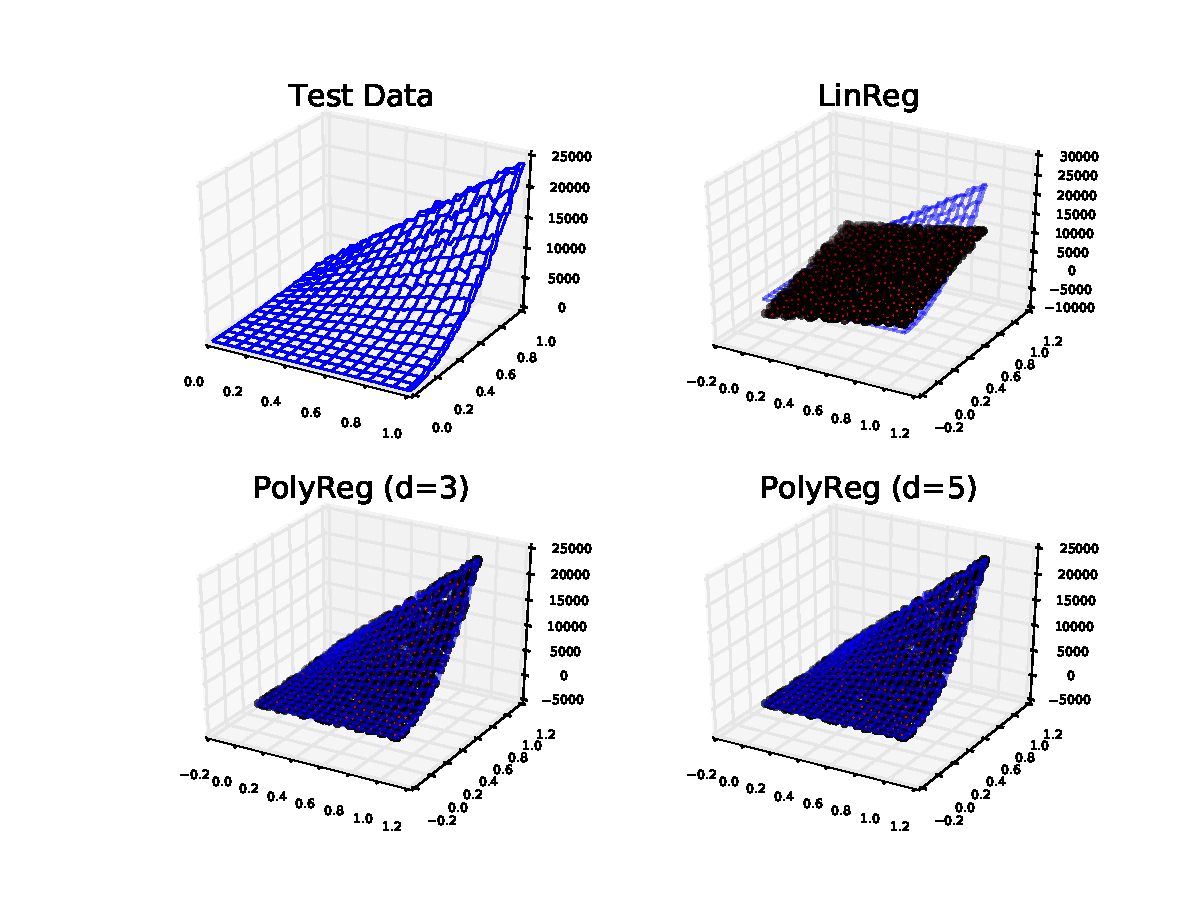
\includegraphics[width=17cm]{plot1.pdf}
\caption{(a) Test data (b) Predictions by Linear Regression (c) Predictions by Polynomial Regression of third degree (d) Predictions by Polynomial Regression of fifth degree}
\label{fig1}
\end{center}
\end{figure}

One can not see from the plot (Figures \ref{fig1}(c) and \ref{fig1}(d)), which polynomial regression model is better, but looking at Table \ref{tab1}, polynomial regression of 3rd order has slightly lower error reported and can be regarded as the best model that fitted data.

\begin{table}[]
\centering
\caption{Result of regression without regularization obtained by the closed form}
\label{tab1}
\begin{tabular}{|l|l|l|}
\hline
\multicolumn{1}{|c|}{\textbf{Closed Form}} & \textbf{Train Error} & \textbf{Test Error} \\ \hline
Linear Regression             & 2.29e+06             & 6.47e+06            \\ \hline
Polynomial Regression (deg=3) & 3.31e-20             & 5.65e-20            \\ \hline
Polynomial Regression (deg=5) & 1.40e-12             & 2.91e-12            \\ \hline
\end{tabular}
\end{table}

\section{Regression without Regularization - Gradient Descent}
In this section, \textit{Gradient Descent} have been used to find the parameters (i.e. weights) of the model, instead of the \textit{closed form} deployed in previous section.

\begin{table}[]
\centering
\caption{Result of regression without regularization obtained by Gradient Descent}
\label{tab2}
\begin{tabular}{|l|l|l|}
\hline
\multicolumn{1}{|c|}{\textbf{Gradient Descent}} & \textbf{Train Error} & \textbf{Test Error} \\ \hline
Linear Regression                               & 2.29e+06             & 6.47e+06            \\ \hline
Polynomial Regression (deg=3)                   & 2.51e-20             & 7.98e-20            \\ \hline
Polynomial Regression (deg=5)                   & 1.33e+01             & 6.79e+01            \\ \hline
\end{tabular}
\end{table}

The stopping criterion for all models is set to max iteration of one million. The learning rate $\eta$ for the first model is set to $10^-6$ and $10^-3$ for the two remaining polynomial regressions. Train and test error for each model is shown in Table \ref{tab2}. As expected, the results are in accordance with Table \ref{tab1} and still suggests the superiority of Polynomial Regression of third degree to the other.

\begin{figure}
\begin{center}
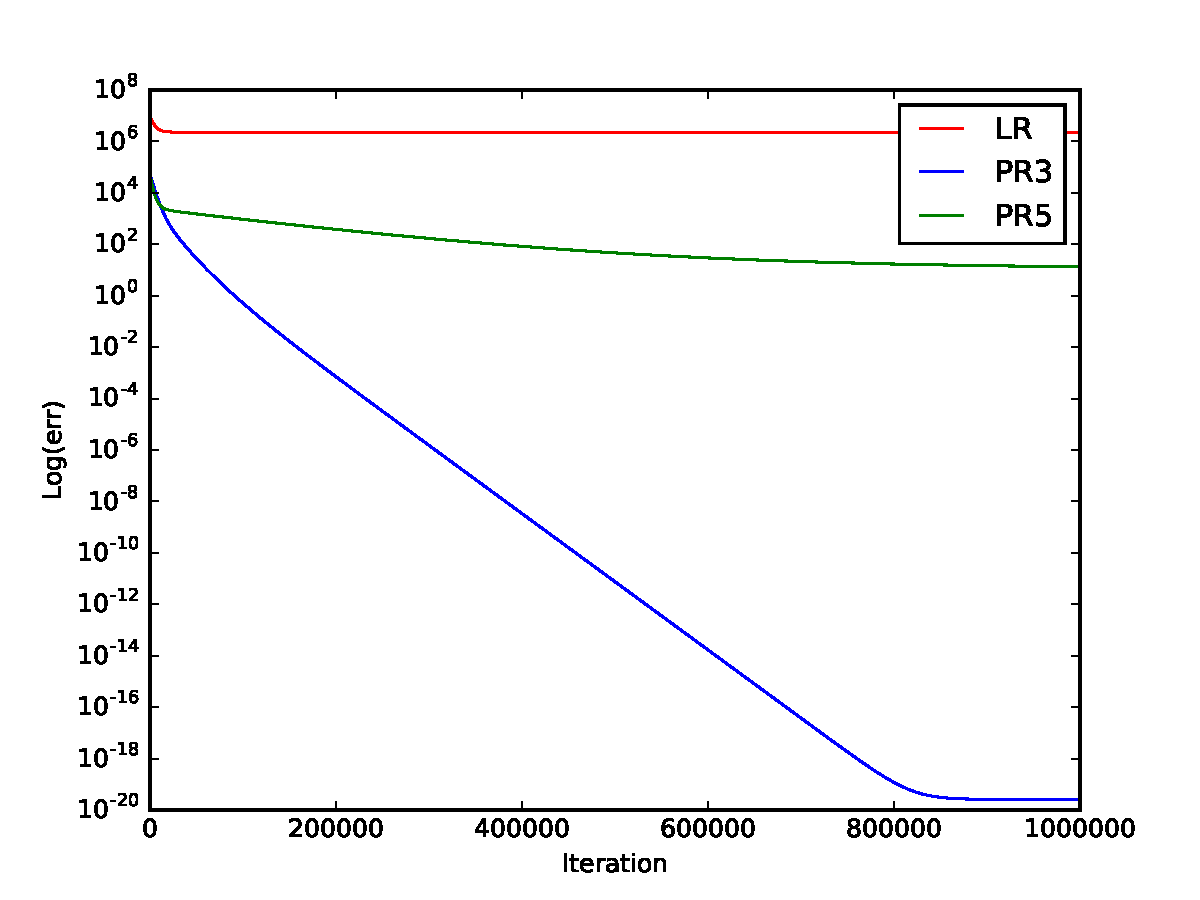
\includegraphics[width=12cm]{plot2.pdf}
\caption{The value of cost function during the training over iterations}
\label{fig2}
\end{center}
\end{figure}

Figure \ref{fig2} depicts how the error calculated by the cost function behaved for these models. The error axis is in logarithmic scale. PR3 has converged after around 800000 iterations to a very minuscule error. Setting the same learning rate for LR would result in its divergence (hence the lower $\eta$). The closed form achieved lower error for PR5, that apparently needs more iterations for this model to be acquired.

It is worth to say that based on empirical results, I have normalized the data beforehand. 

\begin{figure}
\begin{center}
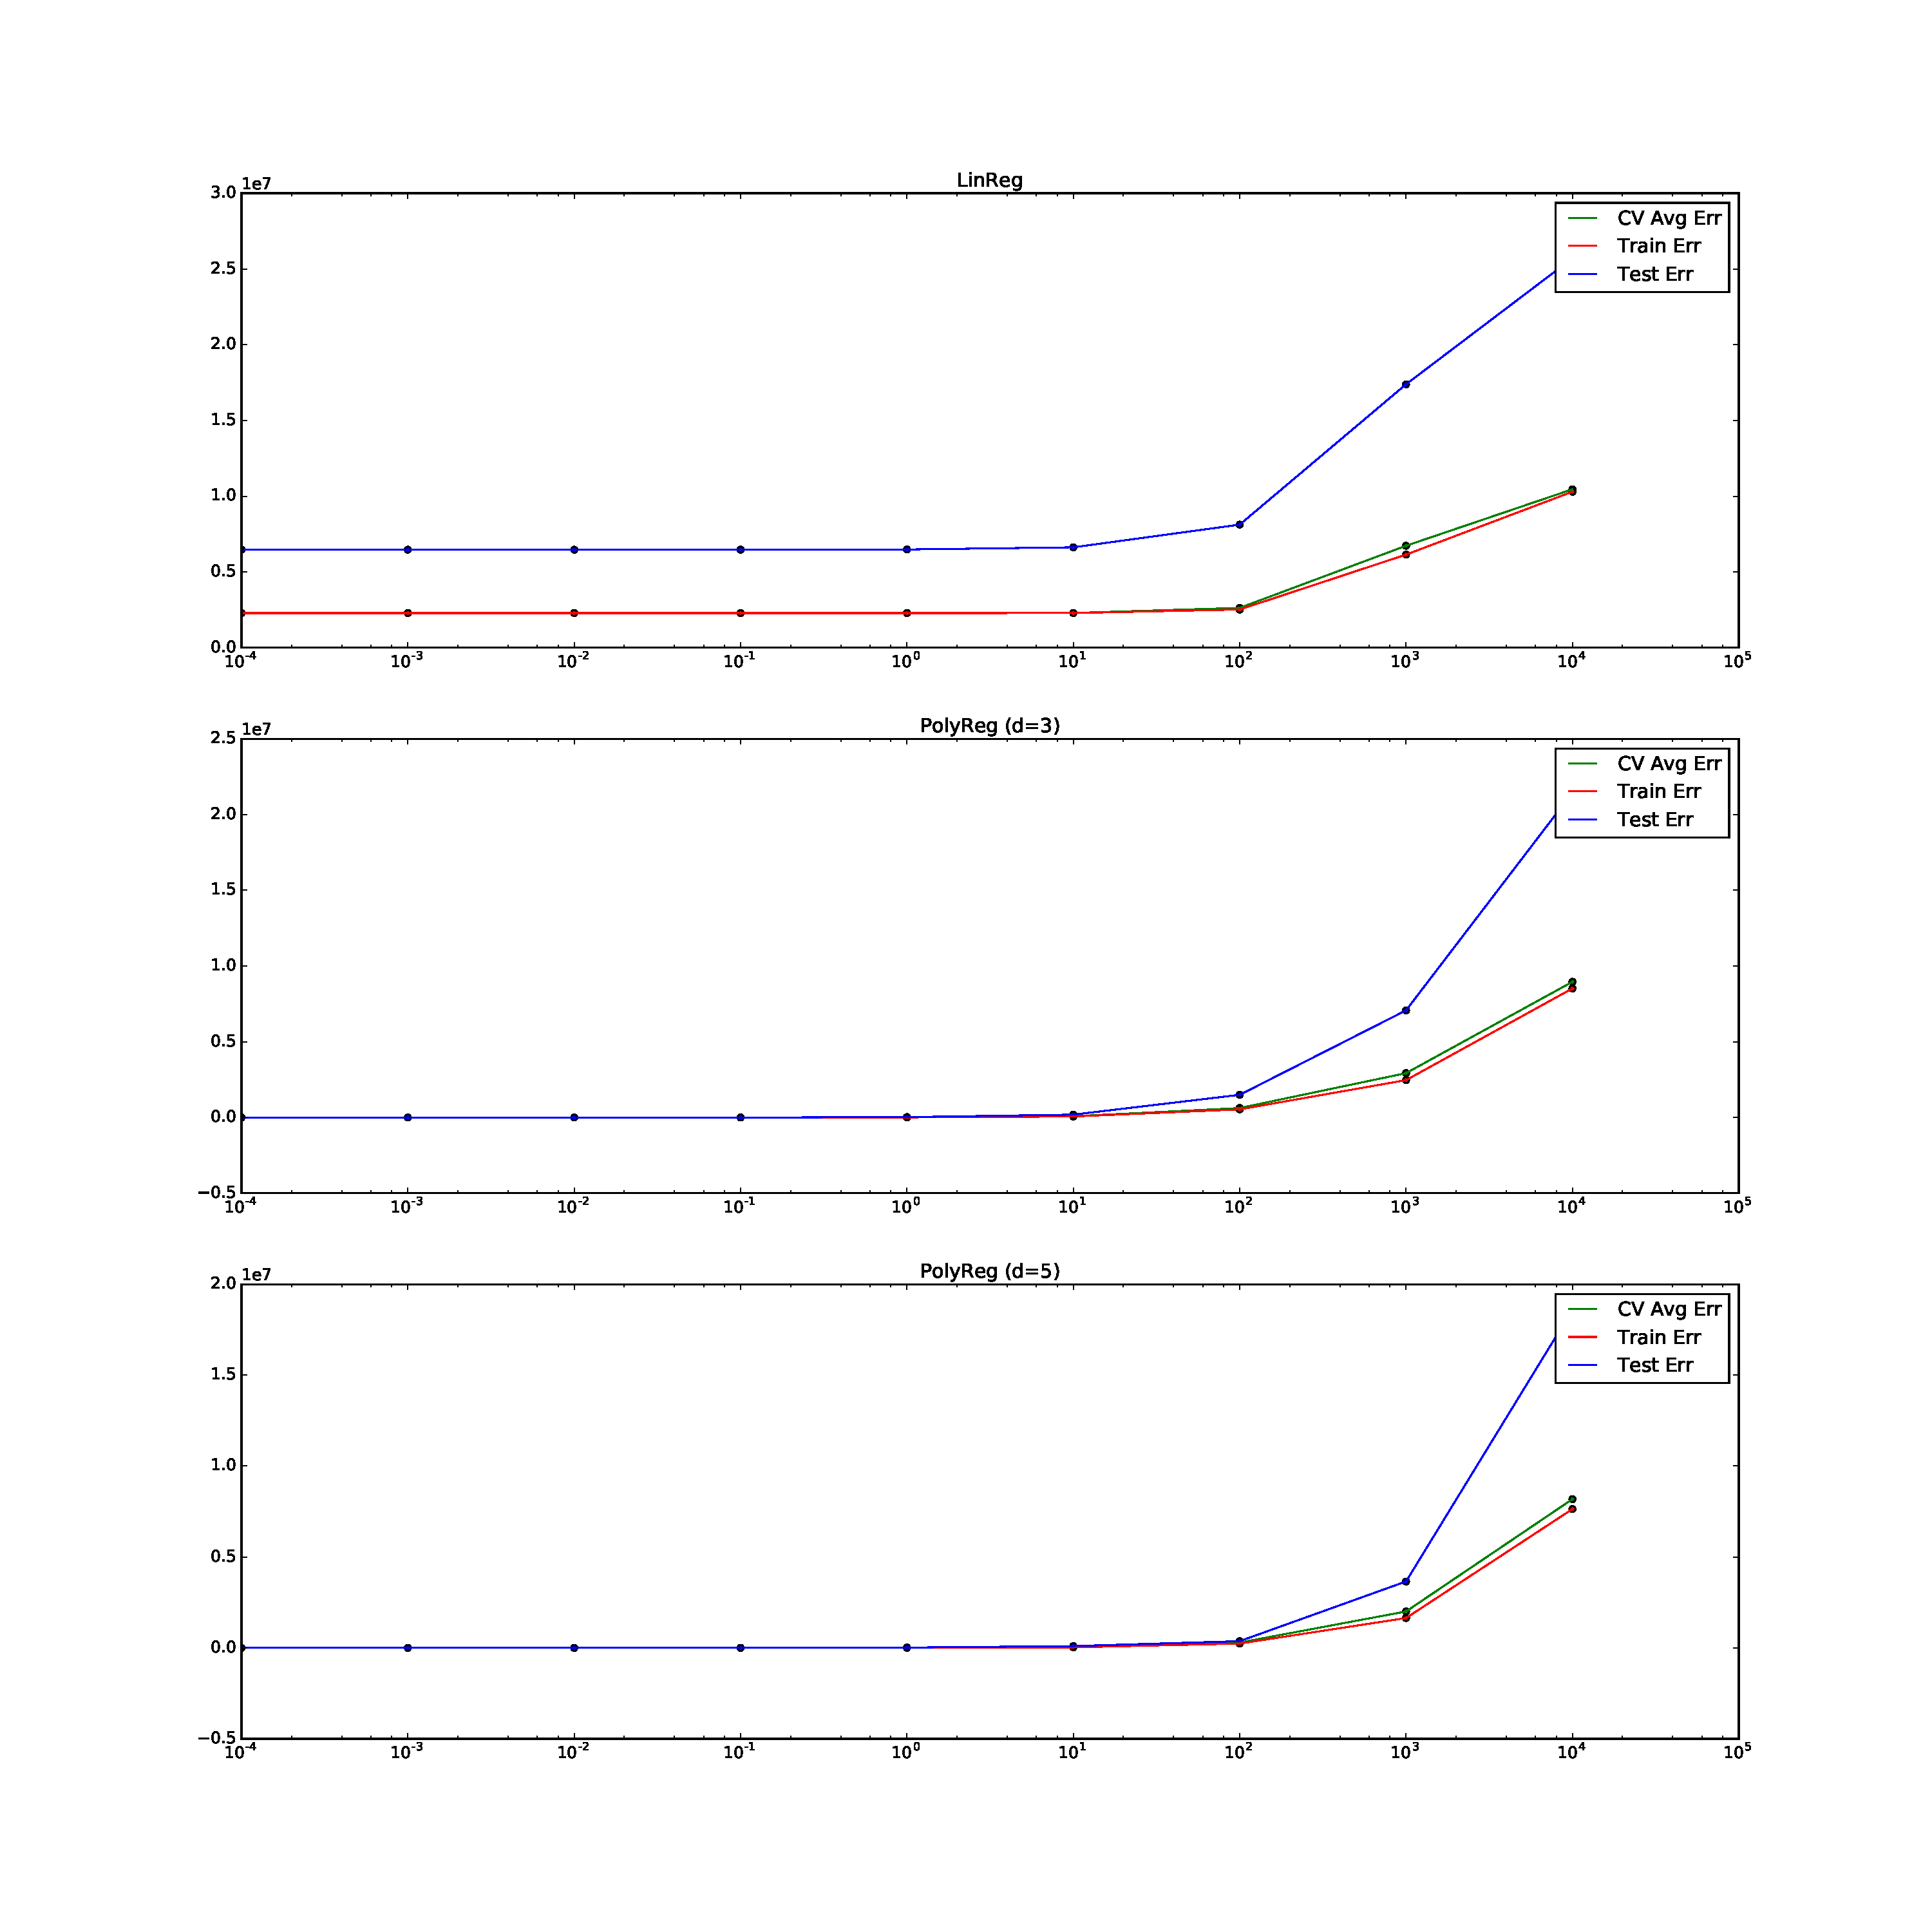
\includegraphics[width=13cm]{plot3.pdf}
\caption{Cost for different values of $\lambda$}
\label{fig3}
\end{center}
\end{figure}

\section{Regression withRegularization - Closed Form}

The best lambda for each models is respectively, 0.1, 0.0001 and 0.0001. Figure \ref{fig3} plots the error value for different regularization parameter $\lambda$.

In each plot in Figure \ref{fig3}, the average of error for prediction performance on held-out validation folds is drawn, along the train and test errors. The figure indicates that cross-validation is a fine strategy to choose the regularization parameter $\lambda$.

\end{document}
